\subsection{Rubidium discharge lamp}

The rubidium discharge lamp consists of three main components : an RF oscillator, an oven,
and a gas bulb. The bulb contains rubidium metal in its naturally occurring isotopic
concentration (28\% $^{87}$Rb and 72\% $^{85}$Rb) together with xenon as a buffer gas.
It sits within the coil of the RF oscillator, as shown in figure below :
 
\begin{figure}[h]
    \centering
    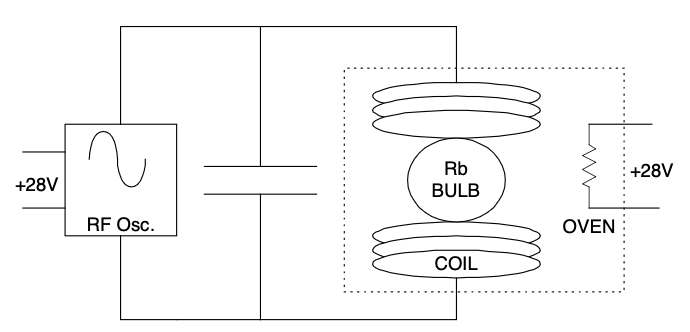
\includegraphics[width=0.55\textwidth]{figures/RB blub.png}
    \caption{Schematic of the rubidium discharge lamp and its back-panel connections.}
    \label{fig:lamp_schematic}
\end{figure}
 
\subsubsection*{Excitation Mechanism}
 
The RF oscillator operates at a frequency of 75--90~MHz with a supply voltage of
$+28$~V~DC. The oscillating magnetic field induces a high electric field inside the bulb,
which ionizes the gas. The resulting free electrons are accelerated and gain kinetic energy :
\begin{equation}
    E_k = eV_{\text{acc}}
    \label{eq:electron_energy}
\end{equation}
Collisions between accelerated electrons and neutral Rb atoms promote the atoms into
excited electronic states. Spontaneous emission from these states produces the rubidium
resonance radiation. The two principal emission lines of interest are :
\begin{equation}
    \lambda_1 = 780\ \text{nm} \quad (^2S_{1/2} \to\, ^2P_{3/2}),
    \qquad
    \lambda_2 = 795\ \text{nm} \quad (^2S_{1/2} \to\, ^2P_{1/2})
    \label{eq:Rb_lines}
\end{equation}
Only the 795~nm line is used in the optical pumping experiment; the 780~nm line is
removed by the interference filter.
 
\subsubsection*{Vapour Pressure and Lamp Intensity}
 
The rubidium vapour pressure determines the atomic number density $\rho$ in the bulb.
From the Clausius-Clapeyron equation, the vapour pressure varies with temperature as :
\begin{equation}
    \ln P = -\frac{L}{R}\cdot\frac{1}{T} + C
    \label{eq:vapour_pressure}
\end{equation}
where $L$ is the molar latent heat of vaporisation and $R$ is the universal gas constant.
The lamp intensity scales approximately linearly with $\rho$ and hence exponentially with
$1/T$. In practice, the lamp intensity increases by approximately 5\% per $^\circ$C at
operating temperature; the oven is therefore stabilised at $120 \pm 2\ ^\circ$C to ensure
a stable output. The photon flux $\Phi$ incident on the absorption cell is :
\begin{equation}
    \Phi = \frac{P_{\text{lamp}}}{h\nu} \cdot \frac{A_{\text{det}}}{4\pi d^2}
    \label{eq:photon_flux}
\end{equation}
where $P_{\text{lamp}}$ is the optical power of the lamp, $A_{\text{det}}$ is the
detector active area, and $d$ is the lamp-to-detector distance.
 
\subsubsection*{Electrical Specifications}
 
The lamp operates with the following nominal parameters :
 
\begin{table}[h]
    \centering
    \begin{tabular}{lc}
        \hline
        Parameter & Value \\
        \hline
        Oscillator supply voltage  & $+28$~V~DC \\
        Oscillator current         & 120--160~mA \\
        Oven supply voltage        & $+28$~V~DC \\
        Oven current (warm-up)     & 350~mA \\
        Oven current (steady state)& 100~mA \\
        Oscillator frequency       & 75--90~MHz \\
        Oven temperature           & $120 \pm 2\ ^\circ$C \\
        Total lamp intensity       & 9.0~$\mu$W \\
        Intensity at 795~nm        & 1.7~$\mu$W \\
        \hline
    \end{tabular}
    \caption{Electrical and optical specifications of the rubidium discharge lamp.}
    \label{tab:lamp_specs}
\end{table}
 
\noindent
The lamp requires 10--20~minutes to reach thermal equilibrium after power is applied.
Note that the 795~nm resonance line lies in the near infrared and is invisible to the
naked eye; the visible purplish-pink glow observed during operation originates from other
rubidium and xenon emission lines.
 